\documentclass[10pt,UTF8]{book} %% ctexart

\title{数据库系统基础}
\author{钱锋\thanks{Email: strik0r\_qf@mail.nwpu.edu.cn}}

\usepackage{ctex}
\usepackage{graphicx}
\usepackage[toc]{multitoc}
\usepackage{booktabs}
\usepackage{longtable}
\usepackage{amsthm, amssymb, amsmath, mathrsfs, mhchem}
\usepackage{tikz,circuitikz}
\usetikzlibrary{decorations.markings, angles, quotes}
\usetikzlibrary{shapes,arrows.meta,positioning}
\usepackage{tikz-cd}
\usepackage{pgfplots}
\usepackage{tikz-3dplot}
\usepackage{extpfeil}
\usepackage{diagbox}
\usepackage{float}
\usepackage{hyperref}
\hypersetup{hidelinks,
    colorlinks = true,
    allcolors = black,
    pdfstartview = Fit,
    breaklinks = true}
\usepackage{caption}
\usepackage{enumitem}
\usepackage{siunitx}
\usepackage{subcaption}
\usepackage{tasks}

\usepackage{fancyhdr} % 用于自定义页眉页脚


% 设置页眉页脚样式
\fancypagestyle{plain}{%
    \fancyhf{} % 清空页眉页脚
    \fancyhead[RO,LE]{·\thepage·} % 页眉显示页码, RO表示奇数页右侧, LE表示偶数页左侧
    \fancyhead[LO]{\nouppercase{\rightmark}} % 页眉显示小节标题, LO表示奇数页左侧
    \fancyhead[RE]{\nouppercase{\leftmark}} % 页眉显示章节标题, RE表示偶数页右侧
    \renewcommand{\headrulewidth}{0.4pt} % 设置页眉横线的宽度
    \renewcommand{\footrulewidth}{0pt} % 取消页脚横线
}

\renewcommand{\headrule}{\hrule width\textwidth height\headrulewidth\vskip-\headrulewidth}

% % 取消奇偶页的页眉偏移
% \fancyhfoffset[RO,LE]{0pt}

% % 取消奇偶页的页眉偏移
% \fancyhfoffset[RO,LE]{0pt}

% 定义取消页眉的命令
\newcommand{\cancelheader}{%
    \fancyhead{} % 清空页眉
    \renewcommand{\headrulewidth}{0pt} % 取消页眉横线
    \renewcommand{\footrulewidth}{0pt} % 设置页脚横线的宽度
}

\renewcommand{\chaptermark}[1]{\markboth{第 \thechapter 章 \hspace{1em} #1}{}}
\renewcommand{\sectionmark}[1]{\markright{\thesection \, #1}}
\usepackage{titlesec} % 定义标题样式

% 设置 chapter 标题样式
\titleformat{\chapter}[hang]{\centering\heiti\Large\bfseries}{第\,\thechapter\,章}{1em}{}

% 定义 section 标题格式
\titleformat{\section}[hang]{\heiti\centering\large\bfseries}{\thesection}{1em}{}

% 定义 subsection 标题格式
\titleformat{\subsection}[hang]{\heiti\bfseries}{\textbf{\thesubsection}}{1em}{}

% 定义 subsubsection 标题格式
\setcounter{secnumdepth}{3}
\renewcommand\thesubsubsection{\arabic{subsubsection}.}
\titleformat{\subsubsection}[hang]{\kaishu}{\quad\quad\thesubsubsection\,\,}{0em}{}

% % 重新定义 textbf
% \let\oldtextbf\textbf
% \renewcommand{\textbf}[1]{{\heiti\oldtextbf{#1}}}

% % 在导言区重新定义 \normalsize 命令
% \makeatletter
% \renewcommand\normalsize{%
%    \@setfontsize\normalsize{10.5pt}{12pt}%
%    \abovedisplayskip 8\p@ \@plus2\p@ \@minus5\p@
%    \abovedisplayshortskip \z@ \@plus3\p@
%    \belowdisplayshortskip 6\p@ \@plus3\p@ \@minus3\p@
%    \belowdisplayskip \abovedisplayskip
%    \let\@listi\@listI}
% \makeatother



% 设置页边距和对齐
% \usepackage[
%     paperwidth=185mm,
%     paperheight=260mm,
%     top=35mm,
%     bottom=25mm,
%     left=18mm,
%     right=18mm,
%     footskip=15mm % 通过这里的值来调整页脚与正文内容的垂直距离
% ]{geometry}

\usepackage[
    paperwidth=210mm,
    paperheight=297mm,
    top=40mm,
    bottom=31.8mm,
    left=25.4mm,
    right=25.4mm,
    footskip=15mm % 通过这里的值来调整页脚与正文内容的垂直距离
]{geometry}

% \usepackage[
%     paperwidth=195mm,
%     paperheight=270mm,
%     top=40mm,
%     bottom=25mm,
%     left=23.5mm,
%     right=23.5mm,
%     footskip=15mm % 通过这里的值来调整页脚与正文内容的垂直距离
% ]{geometry}
\usepackage{mdframed}
\mdfsetup{
  linewidth=0.4pt,
  frametitlebackgroundcolor=white, % 或者 transparent
  frametitlefont=\heiti\bfseries,
  frametitleaboveskip=10pt,
  frametitlebelowskip=5pt,
  frametitlealignment=\raggedright % 新增此行
}
\usepackage{fontspec}
% 设置 Menlo 字体
\setmonofont{Menlo}
\usepackage{fancyvrb}
\usepackage{xcolor}
\usepackage{listings}

\definecolor{string}{HTML}{067D17}
\definecolor{comment}{HTML}{8C8C8C}
\definecolor{keyword}{HTML}{0033B3}
\definecolor{class_field}{HTML}{871094}

\lstset{breaklines}
%这条命令可以让LaTeX自动将长的代码行换行排版
\lstset{extendedchars=false}
%这一条命令可以解决代码跨页时,章节标题,页眉等汉字不显示的问题
\lstset{escapeinside={(*}{*)}}

\lstset{
    basicstyle=\small\ttfamily\heiti,
    numbers=left,
    numberstyle=\scriptsize\fontspec{Menlo}, % 使用 Menlo 字体
    stepnumber=1,
    numbersep=8pt,
    frame=leftline,
    xleftmargin=2em, % 调整代码块的左边界
    framexleftmargin=0pt, % 调整边框的位置
    breaklines=true,
    keywordstyle=\bfseries\color{keyword},          % keyword style
    commentstyle=\heiti\color{comment},       % comment style
    stringstyle=\color[HTML]{067D17},
    showstringspaces=false,
    % string literal style
    % escapeinside={\%*}{*)},            % if you want to add LaTeX within your code
    % morekeywords={}               % if you want to add more keywords to the set
}

\usepackage{smartdiagram} % 表格对角线
\everymath{\displaystyle}
\usepackage{tasks}

\begin{document}
\newtheoremstyle{mytheoremstyle}
    {1.5ex}                                         % Space above
    {1.5ex}                                         % Space below
    {}                                              % Font for body
    {}                                              % Indent amount
    {\bfseries}                                     % Font for head
    {}                                              % Punctuation after head
    {0.5em plus 0.2em minus 0.1em}                  % Space after head
    {\thmname{#1}\thmnumber{ #2}.\thmnote{ (#3).}}

\theoremstyle{mytheoremstyle}
\newtheorem{definition}{定义}[section]
\newtheorem{example}{例}[section]
\newtheorem{exercise}{习题}[section]
\newtheorem{code}{程序清单}[section]
\newtheorem*{result}{运行结果}

\newtheoremstyle{my2theoremstyle}
    {1.5ex}                                         % Space above
    {1.5ex}                                         % Space below
    {\kaishu}                                              % Font for body
    {}                                              % Indent amount
    {\bfseries}                                     % Font for head
    {}                                              % Punctuation after head
    {0.5em plus 0.2em minus 0.1em}                  % Space after head
    {\thmname{#1}\thmnumber{ #2}.\thmnote{ (#3).}}

\theoremstyle{my2theoremstyle}
\newtheorem{thm}{定理}[section]
\newtheorem{law}{定律}[section]
\newtheorem{educt}{推论}
\newtheorem{prop}{命题}
\newtheorem{lemma}{引理}
\newtheorem{axiom}{公理}
\newtheorem{property}{性质}

\newtheoremstyle{my4theoremstyle}
    {1.5ex}                                         % Space above
    {1.5ex}                                         % Space below
    {}                                              % Font for body
    {}                                              % Indent amount
    {\bfseries}                                     % Font for head
    {}                                              % Punctuation after head
    {0.5em plus 0.2em minus 0.1em}                  % Space after head
    {\thmname{#1}.}

\theoremstyle{my4theoremstyle} \newtheorem*{sol}{解}

\newtheoremstyle{my3theoremstyle}
    {1.5ex}                                         % Space above
    {1.5ex}                                         % Space below
    {}                                              % Font for body
    {}                                              % Indent amount
    {\kaishu}                                       % Font for head
    {}                                              % Punctuation after head
    {0.5em plus 0.2em minus 0.1em}                  % Space after head
    {\thmname{#1}\thmnumber{ #2}.\thmnote{ (#3).}}

\theoremstyle{my3theoremstyle} \newtheorem*{remark}{注}
\newtheorem*{cmt}{评注}
% 使用 IEEE 样式
\ctikzset{logic ports=ieee}

\begin{titlepage}
    \thispagestyle{empty}
    \centering
        \vspace*{3cm}
        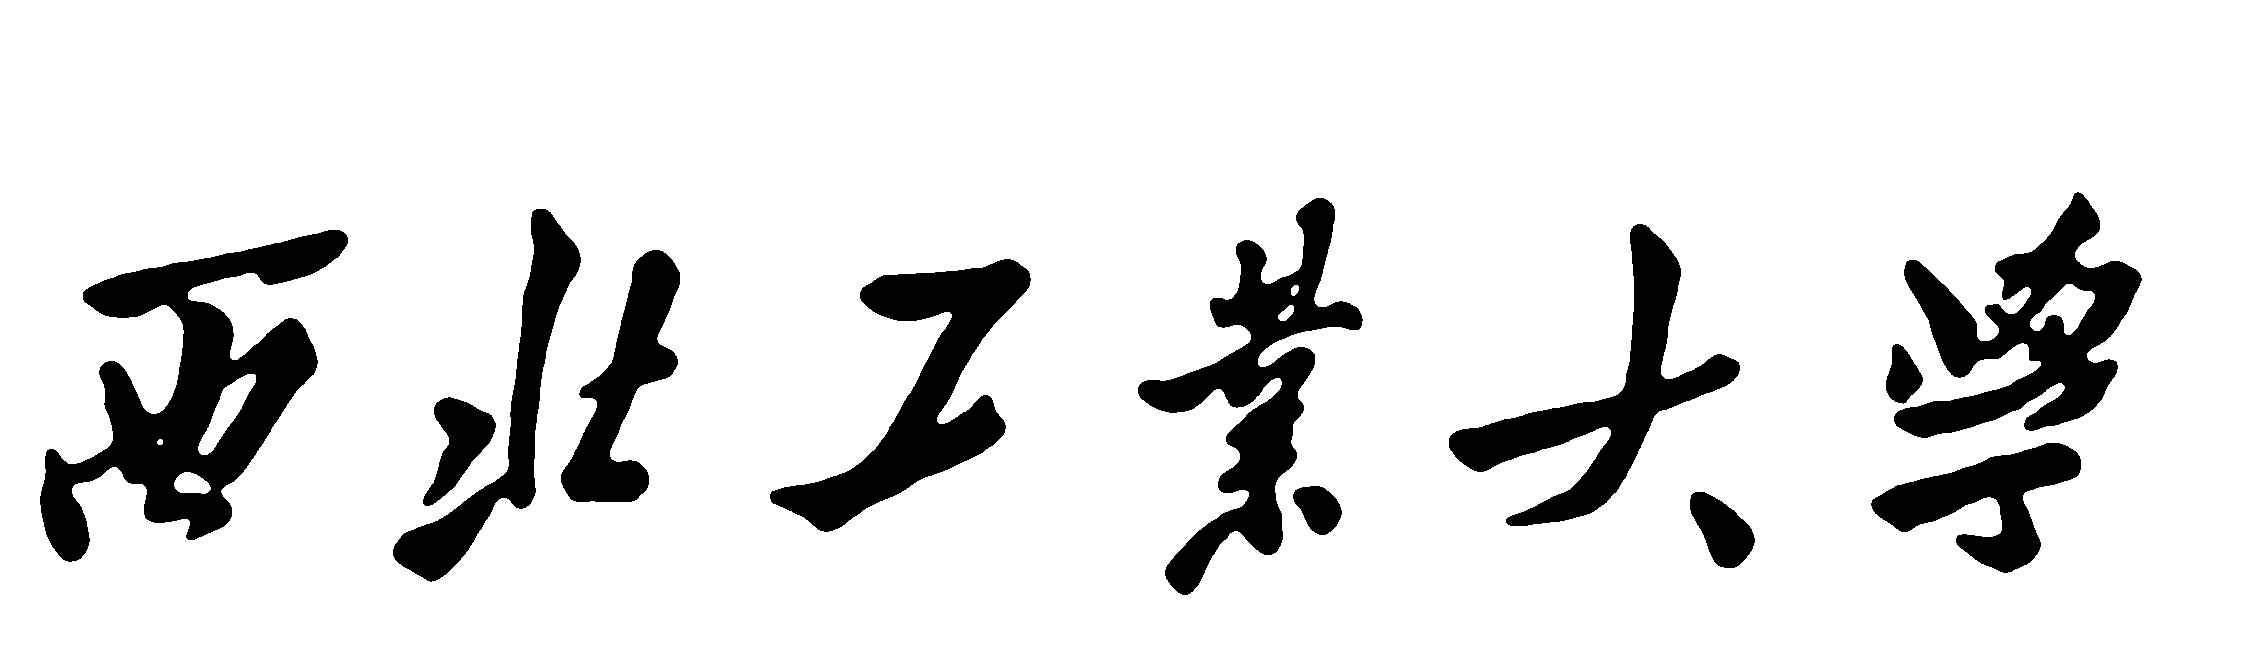
\includegraphics[width=0.5\textwidth]{pic/npu_2.png}\par
        \vspace{1em}
        
\includegraphics[width=0.5\textwidth]{pic/npu_1.png}\par
    \vspace*{1em}
        \begin{center}
            \Huge \heiti \textbf{数据结构习题集}

            Problem Set of Data Structures
        \end{center}

        \vspace{14em}
        \begin{center}
        \songti

        \kaishu 软件学院 \, \heiti\textbf{钱锋} \quad \songti 编
        \vspace{0.5em}

    \today
    \end{center}
\end{titlepage}

\frontmatter
\newpage
\pagestyle{plain}
\makeatother

% 设置目录页的页码格式
\pagenumbering{roman} % 切换回罗马数字页码
\addtocontents{toc}{\protect\thispagestyle{empty}}
\pagestyle{plain}
{\tableofcontents}
\newpage
\thispagestyle{empty}
\cleardoublepage % 确保正文从奇数页开始


% 设置章节标题页的页眉和页脚为空白页样式
\makeatletter
\let\ps@plain\ps@empty
\makeatother

\mainmatter

% \chapter{绪论}
\setcounter{chapter}{1}
\chapter{线性表}

\begin{exercise}
    \begin{enumerate}[itemsep=0pt, label={$\left.\arabic*\right)$}]
        \item 在顺序表中插入或阐述一个元素, 平均需要移动 $n/2$ 个元素, 其中 $n$ 为顺序表当前的
        已使用长度, 具体移动的元素个数与表长和插入元素的目的位置有关.
        \item 顺序表中逻辑上相邻的元素物理位置一定相邻, 但单链表中逻辑上相邻的元素的物理位置未必相邻.
        \item 在单链表中, 除了首元节点外, 任意节点的存储位置有由前驱元素的 \lstinline|next| 指针导出.
        \item 单链表中设置头节点的作用是插入/删除元素时无需进行特殊处理.
    \end{enumerate}
\end{exercise}

\begin{exercise}
    设顺序表中的数据元素递增有序. 试写一算法, 将 \lstinline|x| 插入到
    顺序表的适当位置上, 以保持该表的有序性.
    \lstinputlisting[language=C]{/Users/strik0r/CLionProjects/DataStructure/LinearStructure/LinearList/ProblemSet/2.11-insertElement.c}
\end{exercise}

\begin{exercise}
    试写一算法, 实现顺序表的就地逆置, 即利用原表的存储空间将线性表 $(a_1, a_2, \cdots, a_n)$
    就地逆置.
    \begin{lstlisting}[language=C]
#include <stdio.h>

void reverse(int *arr, int size) {
    int *start = arr; // 指向起始位置的指针
    int *end = arr + size - 1; // 指向末尾位置的指针

    while (start < end) {
        // 交换起始位置和末尾位置的元素
        int temp = *start;
        *start = *end;
        *end = temp;

        // 移动指针
        start++;
        end--;
    }
}

int main() {
    int arr[] = {1, 2, 3, 4, 5};
    int size = sizeof(arr) / sizeof(arr[0]);

    printf("Original array:");
    for (int i = 0; i < size; i++) {
        printf(" %d", arr[i]);
    }
    printf("\n");

    reverse(arr, size);

    printf("Reversed array:");
    for (int i = 0; i < size; i++) {
        printf(" %d", arr[i]);
    }
    printf("\n");

    return 0;
}

    \end{lstlisting}
\end{exercise}

\begin{exercise}
假设有两个按元素值递增有序排列的线性表 \lstinline|A| 和 \lstinline|B| ,均以单链表作存储结
构,请编写算法将 \lstinline|A| 表和 \lstinline|B| 表归并成一个按元素值递减有序(即非递增有序,允许表中含
有值相同的元素)排列的线性表 \lstinline|C|,并要求利用原表(即 \lstinline|A| 表和 \lstinline|B| 表)的结点空间构造 \lstinline|C|
表。
\begin{lstlisting}[language=C]
    #include <stdio.h>
#include <stdlib.h>

// 定义单链表结点
typedef struct Node {
    int data;
    struct Node *next;
} Node;

// 将两个有序链表合并成一个有序链表,递减有序
Node* merge_lists(Node *A, Node *B) {
    Node *C = NULL; // 归并后的链表
    Node *temp;

    // 比较两个链表的节点,将较小的节点插入 C 链表中
    while (A != NULL && B != NULL) {
        if (A->data >= B->data) {
            temp = A;
            A = A->next;
        } else {
            temp = B;
            B = B->next;
        }
        temp->next = C;
        C = temp;
    }

    // 将剩余节点插入到 C 链表中
    while (A != NULL) {
        temp = A;
        A = A->next;
        temp->next = C;
        C = temp;
    }
    while (B != NULL) {
        temp = B;
        B = B->next;
        temp->next = C;
        C = temp;
    }

    return C;
}

// 打印链表
void print_list(Node *head) {
    while (head != NULL) {
        printf("%d ", head->data);
        head = head->next;
    }
    printf("\n");
}

int main() {
    // 初始化两个有序链表 A 和 B
    Node *A = (Node *)malloc(sizeof(Node));
    A->data = 2;
    A->next = (Node *)malloc(sizeof(Node));
    A->next->data = 5;
    A->next->next = (Node *)malloc(sizeof(Node));
    A->next->next->data = 7;
    A->next->next->next = NULL;

    Node *B = (Node *)malloc(sizeof(Node));
    B->data = 3;
    B->next = (Node *)malloc(sizeof(Node));
    B->next->data = 4;
    B->next->next = (Node *)malloc(sizeof(Node));
    B->next->next->data = 6;
    B->next->next->next = NULL;

    printf("原始链表 A:");
    print_list(A);
    printf("原始链表 B:");
    print_list(B);

    // 归并两个有序链表为一个递减有序链表
    Node *C = merge_lists(A, B);

    printf("归并后的链表 C:");
    print_list(C);

    // 释放内存
    while (A != NULL) {
        Node *temp = A;
        A = A->next;
        free(temp);
    }
    while (B != NULL) {
        Node *temp = B;
        B = B->next;
        free(temp);
    }
    while (C != NULL) {
        Node *temp = C;
        C = C->next;
        free(temp);
    }

    return 0;
}

\end{lstlisting}
\end{exercise}

\begin{exercise}
    已知 \lstinline|A|,\lstinline|B| 和 \lstinline|C| 为三个递增有序的线性表,
    现要求对 \lstinline|A| 表作如下操作:删去
那些既在 \lstinline|B| 表中出现又在 \lstinline|C| 表中出现的元素。试对顺序表编写实现上述操作的算法,并
分析你的算法的时间复杂度(注意:题中没有特别指明同一表中的元素值各不相同)。
\begin{lstlisting}[language=C]
#include <stdio.h>
#include <stdlib.h>

// 定义线性表结构
typedef struct {
    int *data;  // 数据域
    int length; // 线性表长度
} SeqList;

// 初始化线性表
void init_list(SeqList *list, int length) {
    list->data = (int *)malloc(length * sizeof(int));
    if (list->data == NULL) {
        printf("内存分配失败\n");
        exit(1);
    }
    list->length = length;
}

// 删除在B表中出现且在C表中也出现的元素
void delete_common_elements(SeqList *A, SeqList *B, SeqList *C) {
    int i = 0, j = 0, k = 0;
    while (i < A->length && j < B->length && k < C->length) {
        if (B->data[j] < A->data[i]) {
            j++;
        } else if (B->data[j] > A->data[i]) {
            i++;
        } else { // B->data[j] == A->data[i]
            if (C->data[k] < A->data[i]) {
                k++;
            } else if (C->data[k] > A->data[i]) {
                i++;
            } else { // C->data[k] == A->data[i]
                // 删除元素
                for (int m = i; m < A->length - 1; m++) {
                    A->data[m] = A->data[m + 1];
                }
                A->length--;
                // 继续比较下一个元素
                j++;
                k++;
            }
        }
    }
}

// 打印线性表
void print_list(SeqList *list) {
    for (int i = 0; i < list->length; i++) {
        printf("%d ", list->data[i]);
    }
    printf("\n");
}

int main() {
    // 初始化线性表 A, B, C
    SeqList A, B, C;
    int length_A = 7;
    int data_A[] = {1, 3, 5, 7, 9, 11, 13};
    int length_B = 6;
    int data_B[] = {3, 6, 7, 10, 11, 14};
    int length_C = 5;
    int data_C[] = {2, 5, 7, 8, 11};
    init_list(&A, length_A);
    init_list(&B, length_B);
    init_list(&C, length_C);
    A.data = data_A;
    B.data = data_B;
    C.data = data_C;

    printf("初始线性表 A:");
    print_list(&A);
    printf("线性表 B:");
    print_list(&B);
    printf("线性表 C:");
    print_list(&C);

    // 删除在 B 表中出现且在 C 表中也出现的元素
    delete_common_elements(&A, &B, &C);

    printf("执行操作后的线性表 A:");
    print_list(&A);

    // 释放内存
    free(A.data);
    free(B.data);
    free(C.data);

    return 0;
}

\end{lstlisting}
该算法首先初始化了三个线性表 \lstinline|A|, \lstinline|B|, \lstinline|C|,并分别存储在数组中。然后使用双指针遍历它们,比较元素大小,删除在 \lstinline|B| 表中出现且在 \lstinline|C| 表中也出现的元素。删除元素的时间复杂度为 $O(n)$,其中 $n$ 为 \lstinline|A| 表的长度。因为该算法涉及对 \lstinline|A| 表的元素进行遍历和删除操作,所以时间复杂度为 $O(n^2)$。
\end{exercise}

\begin{exercise}
    有一个双向循环链表,每个结点中除有 \lstinline|prior|, \lstinline|data| 和 \lstinline|next| 三个域外,还增设了一个访问频度域 \lstinline|freq|。在链表被起用之前,频度域 \lstinline|freq| 的值均初始化为零,而每当对链表进行一次 \lstinline|LOCATE(L,x)| 的操作后,被访问的结点(即元素值等于 \lstinline|x| 的结点)中的频度域 \lstinline|freq| 的值便增 $1$, 同时调整链表中结点之间的次序,使其按访问频度非递增的次序顺序排列,以便始终保持被频繁访问的结点总是靠近表头结点。试编写符合上述要求的 \lstinline|LOCATE| 操作的算法。
    \begin{lstlisting}[language=C]
#include <stdio.h>
#include <stdlib.h>

// 定义双向循环链表的结点
typedef struct Node {
    int data;  // 数据域
    int freq;  // 访问频度域
    struct Node *prior;  // 指向前一个结点的指针
    struct Node *next;   // 指向后一个结点的指针
} Node;

// 初始化双向循环链表
Node* init_list() {
    Node *head = (Node *)malloc(sizeof(Node));
    if (head == NULL) {
        printf("内存分配失败\n");
        exit(1);
    }
    head->data = -1; // 表头结点数据域设为-1
    head->freq = 0;
    head->prior = head;
    head->next = head;
    return head;
}

// 在链表尾部添加结点
void append_node(Node *head, int data) {
    Node *new_node = (Node *)malloc(sizeof(Node));
    if (new_node == NULL) {
        printf("内存分配失败\n");
        exit(1);
    }
    new_node->data = data;
    new_node->freq = 0;
    new_node->prior = head->prior;
    new_node->next = head;
    head->prior->next = new_node;
    head->prior = new_node;
}

// 将结点移动到链表头部
void move_to_head(Node *head, Node *node) {
    node->freq++;
    Node *prev = node->prior;
    Node *next = node->next;

    // 从原位置删除结点
    prev->next = next;
    next->prior = prev;

    // 插入到表头
    node->next = head->next;
    head->next->prior = node;
    head->next = node;
    node->prior = head;
}

// 查找指定值的结点并将其移动到链表头部
void locate(Node *head, int data) {
    Node *current = head->next;
    while (current != head) {
        if (current->data == data) {
            move_to_head(head, current);
            return;
        }
        current = current->next;
    }
    printf("未找到值为 %d 的结点\n", data);
}

// 打印链表
void print_list(Node *head) {
    Node *current = head->next;
    while (current != head) {
        printf("%d(f=%d) ", current->data, current->freq);
        current = current->next;
    }
    printf("\n");
}

int main() {
    Node *head = init_list();

    // 在链表尾部添加一些结点
    append_node(head, 1);
    append_node(head, 2);
    append_node(head, 3);
    append_node(head, 4);
    append_node(head, 5);

    printf("初始链表:");
    print_list(head);

    // 对链表进行 LOCATE 操作
    locate(head, 3);
    printf("执行 LOCATE 操作后:");
    print_list(head);

    locate(head, 5);
    printf("再次执行 LOCATE 操作后:");
    print_list(head);

    // 释放内存
    Node *current = head->next;
    while (current != head) {
        Node *temp = current;
        current = current->next;
        free(temp);
    }
    free(head);

    return 0;
}

    \end{lstlisting}
\end{exercise}

\begin{exercise}
    试以循环链表作稀疏多项式的存储结构, 编写求其导函数的算法,
    要求利用原多项式中的结点空间存放其导函数 (多项式), 同时释放所有无用节点.
    \begin{lstlisting}[language=C]
#include <stdio.h>
#include <stdlib.h>

// 定义多项式的结点
typedef struct Node {
    int coef;  // 系数
    int expo;  // 指数
    struct Node *next;  // 指向下一个结点的指针
} Node;

// 创建空的循环链表
Node *create_empty_poly() {
    Node *head = (Node *)malloc(sizeof(Node));
    if (head == NULL) {
        printf("内存分配失败\n");
        exit(1);
    }
    head->next = head; // 使其指向自己形成循环链表
    return head;
}

// 在多项式的最后添加一个节点
void append_node(Node *head, int coef, int expo) {
    Node *new_node = (Node *)malloc(sizeof(Node));
    if (new_node == NULL) {
        printf("内存分配失败\n");
        exit(1);
    }
    new_node->coef = coef;
    new_node->expo = expo;
    new_node->next = head->next;
    head->next = new_node;
}

// 释放链表的所有结点
void free_poly(Node *head) {
    Node *temp;
    while (head->next != head) {
        temp = head->next;
        head->next = temp->next;
        free(temp);
    }
    free(head);
}

// 打印多项式
void print_poly(Node *head) {
    Node *current = head->next;
    if (current == head) {
        printf("多项式为空\n");
        return;
    }
    while (current != head) {
        printf("%dx^%d ", current->coef, current->expo);
        current = current->next;
        if (current != head) {
            printf("+ ");
        }
    }
    printf("\n");
}

// 求多项式的导函数并存储在原多项式中
void derivative(Node *head) {
    Node *current = head->next;
    Node *prev = head;
    while (current != head) {
        // 计算导数
        current->coef *= current->expo;
        current->expo -= 1;

        // 如果指数为负则删除该节点
        if (current->expo < 0) {
            Node *temp = current;
            prev->next = current->next;
            current = current->next;
            free(temp);
        } else {
            prev = current;
            current = current->next;
        }
    }
}

int main() {
    // 创建一个空的循环链表
    Node *poly = create_empty_poly();

    // 添加多项式的各项
    append_node(poly, 3, 4);
    append_node(poly, -2, 3);
    append_node(poly, 5, 2);
    append_node(poly, 6, 1);
    append_node(poly, -8, 0);

    printf("原多项式: ");
    print_poly(poly);

    // 求导函数
    derivative(poly);
    printf("导函数: ");
    print_poly(poly);

    // 释放内存
    free_poly(poly);

    return 0;
}

    \end{lstlisting}
\end{exercise}

\chapter{栈和队列}

\begin{exercise}
    简述下列算法的功能 (栈的元素类型 \lstinline|SElemType| 为 \lstinline|int|).
    \begin{lstlisting}
Status algo1(Stack S) {
    int i, n, A[255];
    n=0;
    while (!StackEmpty(S)) {n++; pop(S, A[n]);};
    for (i=1; i<=n; i++) Push(S, A[i]);
}
    \end{lstlisting}
    \begin{cmt}
        对栈的操作主要有两种, 分别是入栈 \lstinline|push()|
        和出栈 \lstinline|pop()|, 它们都是对栈顶进行的操作.
        在严蔚敏版数据结构教材 \cite{严蔚敏}
        中, 出栈操作定义为 \lstinline|pop(Stack &S, SElemType &e)|,
        即删除栈顶元素, 并将其值返回到变量 \lstinline|e| 中.
        因此我们不妨用一个例子来直观的叙述该算法的功能.

        假设 $S$ 是一个栈, 它的元素为 $(a, b, c, d)$, 我们约定 $d$ 
        为当前的栈顶, 那么在满足 $S$ 非空时, 我们不断的进行出栈操作,
        并将每一次出栈的元素返回到数组 $A$ 中, 因此这一系列操作中每一步的
        结果是:
        \begin{lstlisting}[language=C]
// 初始状态
S = (a, b, c, d)
A = []

// 出栈
1: S = (a, b, c), A = [NULL, d]
2: S = (a, b),    A = [NULL, d, c]
3: S = (a),       A = [NULL, d, c, b]
4: S = (),        A = [NULL, d, c, b, a]
        \end{lstlisting}
        注意到数组 $A$ 中索引为 $0$ 处实际上是没有元素的,
        在这里我们用 \lstinline|NULL| 来表示这里没有被赋值.
        接下来进行入栈操作, 我们知道当前 $n=4$, $i=1$, 在 $i \leqslant 4$
        的条件下进行循环来实现将数组中的元素按顺序压入栈中:
\begin{lstlisting}
// 入栈
1: S = (d),          A = [NULL, d, c, b, a]
2: S = (d, c),       A = [NULL, d, c, b, a]
3: S = (d, c, b),    A = [NULL, d, c, b, a]
4: S = (d, c, b, a), A = [NULL, d, c, b, a]
\end{lstlisting}
        不难发现该算法的功能实际上就是反转一个栈中的元素.
    \end{cmt}
\begin{lstlisting}
Status algo2(Stack S, int e) {
    Stack T; int d;
    initStack(T);
    while (!StackEmpty(S)) {
        Pop(S, d);
        if ( d != e ) Push(T, d);
    }
    while (!StackEmpty(T)) {
        Pop(T, d);
        Push(S, d);
    }
}
\end{lstlisting}
\begin{cmt}
    这个算法首先初始化了一个空栈 $T$, 然后通过循环将 $S$ 所有的元素全部
    出栈并将不等于 $e$ 的出栈元素压入 $T$ 中. 然后又从 $T$ 中将所有的元素
    出栈并压入 $S$ 中. 注意到由于栈 ADT 的后进先出原则, 因此每次的全部出栈 (all pop)
    操作都会导致元素顺序的完全颠倒, 根据组合数学的知识知道,
    一个排列的完全逆排列的完全逆排列
    就是这个排列本身, 因此 all pop 两次则将恢复原来的顺序,
    因此 栈 $S$  在该算法执行前后唯一的不同就是其中所有的元素 $e$
    都被删除了. 因此该算法的功能是删除栈中的所有等于 $e$ 的元素.
\end{cmt}
\end{exercise}

\begin{exercise}
    假设以 \lstinline|S| 和 \lstinline|X| 分别表示入栈和出栈的操作,
    则初态和终态均为空栈的入栈和出栈操作序列可以有 \lstinline|S|
    和 \lstinline|X| 所完全表达. 我们称可以操作的序列为合法序列
    (例如, \lstinline|SXSX| 是合法序列, \lstinline|SXXS| 为非法
    序列). 试给出区分给定序列是否合法的一般准则, 并证明: 
    对于同一输入序列, 两个不同的合法序列不可能得到相同的输出序列.
    \begin{cmt}
        我们知道, 对于栈操作来说, 如果对空栈进行出栈操作, 那么就会引发
        异常, 因此{\kaishu 栈操作的第一个操作不能为出栈, 最后一个操作不能为入栈}, 
        同时,
        由于栈操作序列的终态为空栈, 因此 {\kaishu 入栈操作和出栈操作的数量
        是相等的}. 更进一步的, 对于任意时刻来说, 为了保证能够有元素出栈,
        {\kaishu 入栈操作的数量与出栈操作的数量非负, 并且对于入栈操作和出栈操作
        数量相等的操作序列, 下一个操作必为入栈操作}.
        基于上述准则, 我们能够判断操作序列的合法性.
    \end{cmt}
    \begin{proof}
        给定入栈序列 $a_1, a_2, \cdots, a_n$, 不妨假设这 $n$ 个元素互不相等
        (这是因为如果存在重复的元素, 那么我们可以构造一些极端的例子, 
        例如 $n$ 个操作是完全相同的元素, 如此一来任何合法操作序列的输出序列都是
        完全相同的), 给定操作序列与
        $o_1, o_2, \cdots, o_n, o_{n+1}, \cdots, o_{2n}$,
        其中 $n$ 个入栈操作, $n$ 个出栈操作.
        我们能够确定长度为 $n$ 的入栈序列所对应的操作总数一定是 $2n$, 是因为
        为了保证初态和终态均为空栈.
        不妨设操作序列 A 和 B 的前 $k$ 个操作是完全相同的, 因此它们的出栈序列
        也是相通的, 此时栈中的元素为
        $a_1a_2\cdots a_m$, 不妨设 A 进行入栈操作 \lstinline|S|, 
        而 B 进行出栈操作 \lstinline|X|,
        则栈中的元素将会变成 $a_1a_2\cdots a_m a_{m+1}$ 和 
        $a_1a_2\cdots a_{m-1}$, 此时 B 的出栈序列中将会新增一个 $a_m$,
        要保证出栈序列相同, 需要在 A 的出栈序列中的对应位置处也得到一个 $a_m$, 而这是不可能的,
        因为由于栈的后进先出特性, 
        为了得到 $a_m$, 必须先把 $a_{m+1}$ 出栈, 而这势必会造成出栈序列的
        不同. 无论 $m$ 取 $2,3,4,\cdots,2n-1$, 这都是成立的.
    \end{proof}
\end{exercise}

\appendix
% 设置 chapter 标题样式
\titleformat{\chapter}[hang]{\centering\heiti\Large\bfseries}{附录\,\thechapter}{1em}{}
\renewcommand{\chaptermark}[1]{\markboth{附录 \thechapter\, #1}{}}

\onecolumn
\begin{thebibliography}{1}
    \addcontentsline{toc}{chapter}{参考文献}
    \bibitem{Mark}
    [美] Mark Allen Weiss. 数据结构与算法分析—— C 语言描述 (原书第 2 版)
    (典藏版) = Data Structures and Algorithm Analysis in C,
    Second Edition [M]. 冯舜玺译. 北京: 机械工业出版社, 2019.
    \bibitem{Michael}
    [美] Michael Goodrich, [美] Roberto Tamassia, 
    [美] Michael H. Goldwasser. 数据结构与算法: Python 语言实现
    = Data Structures and Algorithms in Python [M].
    张晓等译. 北京: 机械工业出版社, 2018.
    \bibitem{Cormen}
    [美] Thomas H. Cormen, [美] Charles E. Leiserson,
    [美] Ronald L. Rivest, [美] Clifford Stein.
    算法导论 (原书第 3 版) = Introduction to Algorithms, Third Edition [M].
    殷建平等译. 北京: 机械工业出版社, 2013.
    \bibitem{耿国华}
    耿国华等. 数据结构: 用 C 语言描述 (第 2 版) [M].
    北京: 高等教育出版社, 2015.
    \bibitem{王道数据结构}
    王道论坛组. 2024 年数据结构考研复习指导 [M]. 北京: 电子工业出版社, 2022.
    \bibitem{严蔚敏}
    严蔚敏, 李冬梅, 吴伟民. 数据结构: C 语言版: 双色版: 第 2 版 [M].
    北京: 人民邮电出版社, 2022.
    \bibitem{习题解析与实验指导}
    李冬梅, 田紫微. 数据结构习题解析与实验指导: 第 2 版 [M]. 北京: 人民邮电出版社, 2022.
\end{thebibliography}


\newpage
\thispagestyle{empty}
\vspace*{5cm}
\begin{center}
    \includegraphics*[width=\textwidth]{pic/i_love_npu.jpeg}
    \large
    公诚勇毅 \quad 永矢毋忘

    中华灿烂 \quad 工大无疆
\end{center}
\vspace*{13em}
\begin{center}
    \small
    本文档由\textbf{钱锋}编写, 钱锋保留一切权利.

    文档中出现的部分素材来源于网络, 笔者承诺这些素材仅供学习交流之用, 
    它们的原作者保留一切权利.

    2023 年 \quad 西北工业大学 \quad 中国西安 
\end{center}

\end{document}